\documentclass{sig-alternate-05-2015}
\usepackage{enumerate}
\usepackage{graphicx}
\usepackage{svg}
\usepackage{url}
\usepackage{amsmath}
\begin{document}

% Copyright
\setcopyright{acmcopyright}
%\setcopyright{acmlicensed}
%\setcopyright{rightsretained}
%\setcopyright{usgov}
%\setcopyright{usgovmixed}
%\setcopyright{cagov}
%\setcopyright{cagovmixed}


\title{SmartPhone based Sound Direction Estimation}

%

\numberofauthors{1} %  in this sample file, there are a *total*
% of EIGHT authors. SIX appear on the 'first-page' (for formatting
% reasons) and the remaining two appear in the \additionalauthors section.
%
\author{
% You can go ahead and credit any number of authors here,
% e.g. one 'row of three' or two rows (consisting of one row of three
% and a second row of one, two or three).
%
% The command \alignauthor (no curly braces needed) should
% precede each author name, affiliation/snail-mail address and
% e-mail address. Additionally, tag each line of
% affiliation/address with \affaddr, and tag the
% e-mail address with \email.
%
% 1st. author
\alignauthor
Amit Sharma, Youngki Lee, Rajesh K Balan, Archan Misra\\     
       \affaddr{Singapore Management University}\\
       \affaddr{Singapore}\\
       \email{\{amit.2015, youngkilee, rajesh, archanm\}@smu.edu.sg}
}
% There's nothing stopping you putting the seventh, eighth, etc.
% author on the opening page (as the 'third row') but we ask,
% for aesthetic reasons that you place these 'additional authors'
% in the \additional authors block, viz.




% Just remember to make sure that the TOTAL number of authors
% is the number that will appear on the first page PLUS the
% number that will appear in the \additionalauthors section.

\maketitle
\begin{abstract}
Information about sound direction can be quite useful in certain situations. For example, imagine a lecture hall with video recording facility. We want to video record the speaker along with attendants asking questions, if any. Using a smartphone, we can detect direction of current speaker and accordingly automatically rotate the camera to capture the speaker. Another application could be assistance to a deaf person in a meeting. Since they rely on lip/gesture reading of the speaker to understand the ongoing discussion, so a smartphone can be used to detect the speaker direction and help the deaf person look in appropriate direction.\\

In this work, we present our sound direction estimation application that exploits Time Difference of Arrival (TDOA) of two signals at two microphones of a smartphone and signal cross-correlation for angle estimation. We used only one smartphone with two microphones to detect directions from 0 to 180 degrees. Experiment results for using \textit{white noise} as a sound source are discussed in this work. Our approach can detect 37 different angles for a smartphone with microphones 14 cm from each other.

\end{abstract}


\keywords{SmartPhone, Time-differnce of Arrival (TDOA), Angle of Arrival, Cross-Correlation}

\section{Introduction}
Detecting direction of speaker can be quite useful in small gatherings e.g. meetings and seminars. Since smartphones are getting more and more pervasive day by day, so smartphone based sensing applications are quite useful.  Consider a scenario wherein a deaf person is attending the meeting. He relies on lip/gesture reading of the speaker to understand what is being discussed. In order to be able to lip-read the speaker, it is important for him to know where to look for the speaker. So, real-time direction detection becomes quite critical here. If the person happen to have a smartphone, then it can be used to estimate the direction of the sound and the person can just look at the smartphone to find out where to look for the speaker.

Another possible application could be in camera automation e.g. a video camera in a conference room can be automatically rotated to capture the speaker as well as audience if they also participate in discussion. For this, we need to install actuators on the camera and attach a smartphone with the camera. Depending on the angle detected by the Smartphone, actuators can rotate the camera accordingly.

Direction of the speaker can be detected using multiple microphones or microphone array as described in \cite{everydaysounds} [cite papers here]. But, this requires a dedicated setup of microphone hardware which is not possible to carry around all the time especially in above described scenarios.

Smartphones on the other hand are always carried by the people. Many of the smartphones have more than one microphones available on-board which potentially can be used for sound direction detection. Since these microphones are located at different positions and are separated by some distance, so the signals received at both the microphones can differ in amplitude and time of arrival depending on the position of source.This difference in amplitude and time of arrival can be used to estimate the direction of incoming sound. We have developed an Android application which leverage two microphones available on a smartphone to provide a real-time estimate of sound direction. Two microphones on the smartphone can capture two separate audio signals in stereo recording mode. We compute difference in time of arrival of these two signals at the two microphones to estimate angle of arrival of the sound source. Using signal convolution, we find lag between the two received sound sample arrays, then simply using cosine law, angle of arrival is estimated. All processing is done on smartphone itself and hence no cloud connectivity is required. Also, our method doesn't require any sort of signal processing and we don't need to store the incoming sound stream to phone memory, the analysis is done directly on the incoming data stream. Since the sound source can be either white noise or human voice etc., so in this paper, we discuss the results of our experiment with white noise as the sound source.




%\section{Related work}

\section{system design}
We have developed an Android application, DirectionDetector, which provides an interface to start/stop the angle estimation process. The application interface displays the estimated angle with respect to the camcorder microphone (the one closer to the camera). Figure ~\ref{fig:screenshot} [insert a figure number here] shows the screenshot of the application. [?????? add a figure that shows the way of angle measurement visually].

\begin{figure}
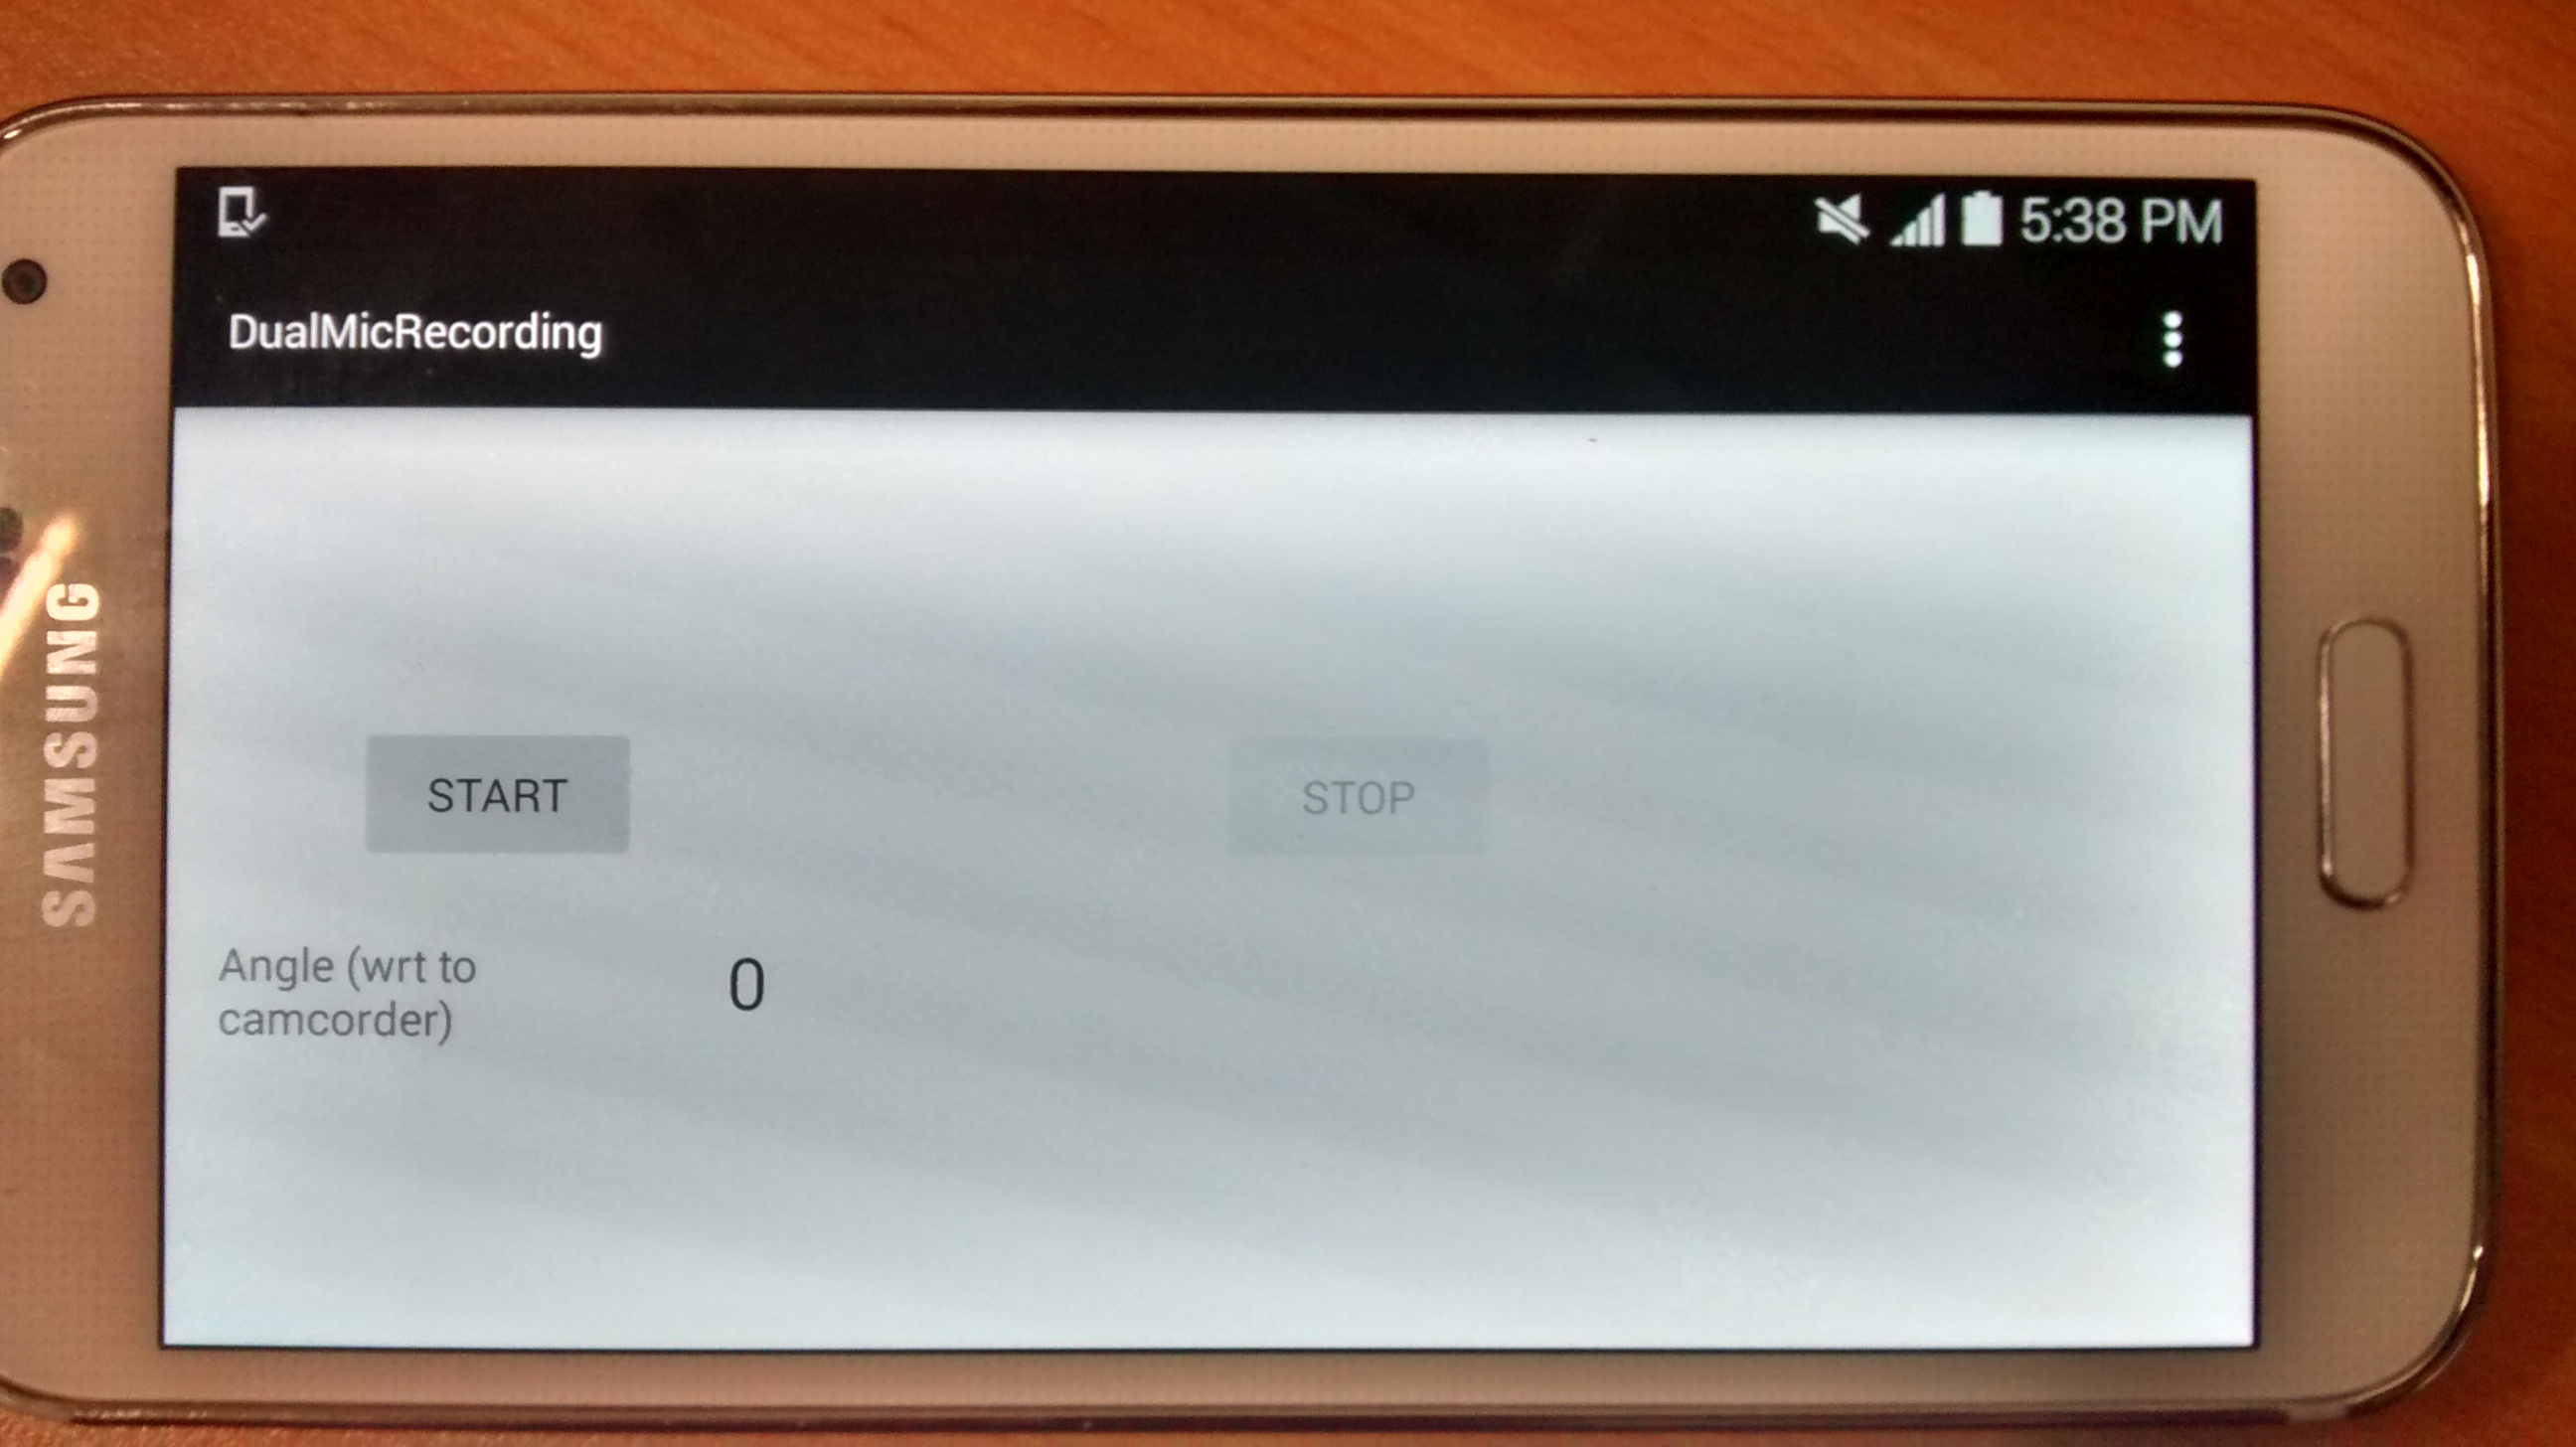
\includegraphics[width=90mm, height=60mm]{figures/screenshot.jpg}
\caption{Android Application Screenshot}
\label{fig:screenshot}
\end{figure}


\begin{figure}
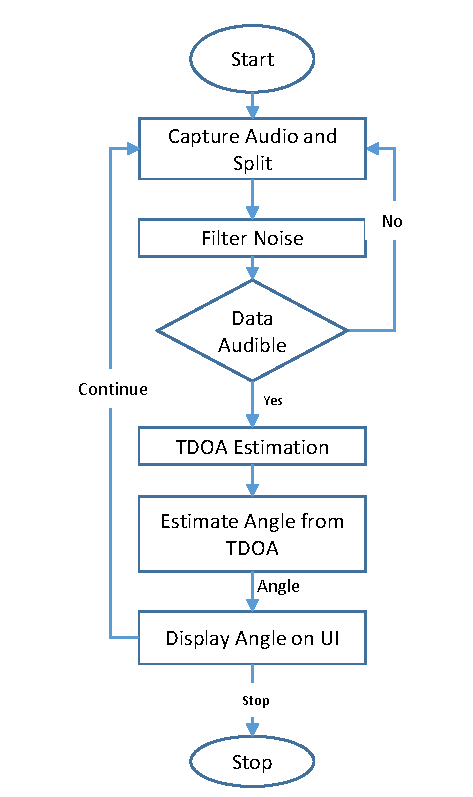
\includegraphics[width=80mm, height=100mm]{figures/flowchart.pdf}
%\includesvg{figures/flow_chart.svg}
\caption{Flow Chart of Angle Estimation}
\label{fig:flowChart}
\end{figure}

The flow chart in Figure ~\ref{flowChart} represents the steps involved in angle estimation. Once the user starts the detection process, by clicking on start button on application interface, the application start capturing sound samples from both the microphones i.e. camcorder and mic. The sampling rate can be varied from 8000 HZ to 44100 HZ. For our experiments, we used 44100 HZ because Android guarantees to support this sampling rate at all devices and also using higher frequency provides a better estimate. Each step of flow chart is explained below.
\subsection{Capture Audio \& Split }
When recording audio in stereo mode, Android puts captured audio frames from both the microphones in one single buffer. Frames at even indices belong to one channel and those at odd indices belong to another channel. For processing, the application can read data from this system buffer and then split frames for both channels. In our analysis we read 4096 samples at a time from Android buffer and before proceeding further, we split this array into two different vectors, one for \textit{camcorder} data and other for the \textit{mic} data. Elements of these arrays are called frames of audio data. Individual frames are processed for angle estimation. 

\subsection{Noise filter}
Since the environment may have some ambient noises, so before estimating angle for captured samples, we filter the possible noise. We compute root mean square value of sound magnitude. If this magnitude is lower than a certain threshold, then these samples are not used for angle estimation and rather discarded. Samples with root mean square value above the threshold are passed to the angle estimation module. Also, some smartphones might have an inbuilt noise suppressor module, so on devices with that capability, we use noise suppressor module together with our noise filter to filter samples in better way.

\subsection{TDOA estimation}
The objective of this step is to estimate TDOA of both signals. The time difference might arise because microphones might be at different distances from the sound source. Given two audio signals,   cross-correlation can be used for lag estimation. The idea behind this approach is that two similar audio signals would have maximum correlation. Sum of the products of frames in camcorder and mic vectors will be maximum when both signals are similar. So, given camcorder and mic data array, we shift the frames of mic array and compute sum of products of frames of both arrays for this shift. Each shift corresponds to a lag in terms of delay in number of audio frames with respect to camcorder. For example, we start by left shifting elements of mic array by N. For this shift, sum of products of elements of camcorder and mic array is computed and  stored. This represents correlation value corresponding to lag equal to -N . This negative lag means that mic samples lag behind camcorder samples by N number of frames. Similarly, we compute correlation value for left shift equal to N-1 and store it. This process is carried on for N times for left shift followed by N times for right shift. We also compute sum of products for 0 lag. The value of N is dependent on distance between two microphones and the sampling frequency. The formula for N is given below.

\begin{gather*}
N =  \frac{d} {v} *S
\end{gather*}

Here, d represents the distance between two microphones, v is sound velocity in air (343 m/s) and S is sampling frequency. From all these correlation values for different lags, we pick the maximum value and record the lag corresponding to that value. This lag value is actually lag in terms of number of frames, so we divide it with sampling frequency to calculate TDOA which represents difference in time-of-arrival in seconds.

For value of d equals 0.14 meter and S equals 44100 Hz, the value of N comes out to be 18. So, we can shift our signal vectors from -18 to +18 resulting in 37 possible values of lag. Since each lag value can be mapped to an angle of arrival, so this technique can estimate 37 different angles in 0 to 180 degrees.


\subsection{Compute angle from TDOA}
Once we have TDOA, we estimate angle of arrival from it. The angle of arrival derivation looks like as shown in Figure ~\ref{fig:aoaDerivation}. In this figure, the sound source lies somewhere in first quadrant and the inclined straight lines represents sound waves coming from the source. Left red cross corresponds to camcorder and right cross to mic of smartphone. Value of d represents the distance between camcorder and mic measured in meters, $d_T$ represents difference in distance travelled by each audio frame to reach both the microphones, $v_2$ represents sound velocity in air and $\theta$ represents the angle of arrival with respect to camcorder of the smartphone. After estimating TDOA in previous step, we can compute  $d_T$ using velocity of sound in air (343m/s). Once all these values are computed then $\theta$ can be computed by following formula.
\begin{gather*}
\theta = \cos^{-1}(\frac{v_2 * TDOA}{d})
\end{gather*}


Value of angle from this equation can vary from 0 to 90 degree because of right angle triangle. So, in order to estimate angle of arrival for sound source in second quadrant, we use sign of lag. If lag value is negative then the sound source is in second quadrant (closer to camcorder) and if it is positive, then sound source lies in first quadrant (closer to mic). So, for a given value of lag, we compute angle using its absolute value and then using the sign of lag, we estimate we estimate the actual angle. For lag < 0, the angle is 180 - $\theta$ and for lag >=0 the angle is $\theta$.

Since position of microphones may vary device to device, so we need to manually measure the distance between microphones. For our experiments, we used Samsung Galaxy S5 with value of d equals to 0.14 meters.

\begin{figure}
\centering
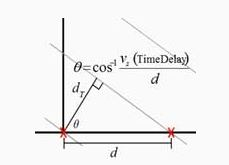
\includegraphics{figures/angle-of-arrival.jpg}
\caption{Angle of Arrival derivation ~\protect\cite{derivationSource}}
\label{fig:aoaDerivation}
\end{figure}

%This approach can be used for angle estimation from 0 to 180 degrees only and hence the application wouldn't be able to differentiate sound sources in first and third quadrants with same TDOA values. Similarly, it is not feasible to differentiate between sources in second and fourth quadrants with same values of TDOA. We believe that if a smartphone has a third microphone (many high end smartphones have 3 microphones), then we can remove this limitation and then this same approach can be used to detect angles from 0 to 360 degress.

\subsection{Display angle on UI}
Using the steps above, SoundDetector estimate angles to be displayed to the user. But before displaying, we need to apply a smoothing algorithm because sometimes temporary/sudden ambient noises causes interference leading to wrong angle prediction. So, it is important to minimize effects of these noises. Our smoothing algorithm is based on counting frequency of each estimated angle and then the final angle is the one with highest frequency. All estimated angles are recorded in a vector of length \textit{smoothing\_window} (equal to 10 in our experiments) and then the angle which was seen most frequently is displayed on the UI. Angle computation and display occurs on two separate threads. 


\section{experiment setup}
For computing the accuracy of our system, we collected audio samples from sound source at different angles (0, 30, 45, 60, 90, 120, 135, 150, 180). Multiple samples [how many????????????] were collected from each position. Then we compared the estimated angle with the ground truth giving us the accuracy of angle estimation by our system. It is interesting to study if distance between sound source and the smartphone has any impact on the accuracy of angle estimation. So, we also varied distance between the source and smarpthone from 1 meter to 2 meters and 3 meters. For each value of distance, we collected multiple samples from each angle and estimated angle for each sample. 

Experiments were done inside a meeting room [dimensions please????????????] with very low noise (low ambience noise). The sound used for the experiment is a white noise [cite it please ?????????]. The selection of specific music is arbitrary and angle estimation is independent of type of white noise chosen.

The smarpthone used for experiments is Samsung S5 running Android v4.4.2 (kitkat) with 2 GB of RAM and quad-core 2.5 GHz of CPU clock. This smartphone has one microphone at the top and the other at the bottom.

\section{Results}

\section{Future work}
Our current approach uses only two microphones for angle estimation. If one choose two symmetric points in first and third quadrants with same value of TDOA, then the system although will determine the angle correctly but would not be able to differentiate between first and third quandant. So future work would focus on using a smartphone with three microphones and use received sound amplitude to differentiate between sources in first-third and second-fourth quadrants. Using a third microphone, we can extend our technique to estimate angles from 0 to 360 degrees.

Secondly, the current implementation doesn't consider the height of the sound source and all the estimation assumes the sound source to be on same level as the smartphone. If smartphone and sound source are at different heights then the estimated angle might have an error. In our future work, we plan to introduce height as another parameter for angle estimation. 

Lastly, we believe it would be interesting to see a comparison of accuracy between different sources of sound. Current implementation uses white noise as sound source, the future implementation would also consider other sound sources e.g. human voice.



\nocite{4459286}
% produce the bibliography for the citations in your paper.
\bibliographystyle{abbrv}
\bibliography{biblio}  % sigproc.bib is the name of the Bibliography in this case

% You must have a proper ".bib" file
%  and remember to run:
% latex bibtex latex latex
% to resolve all references
%
% ACM needs 'a single self-contained file'!
%
%APPENDICES are optional
%\balancecolumns

\end{document}
